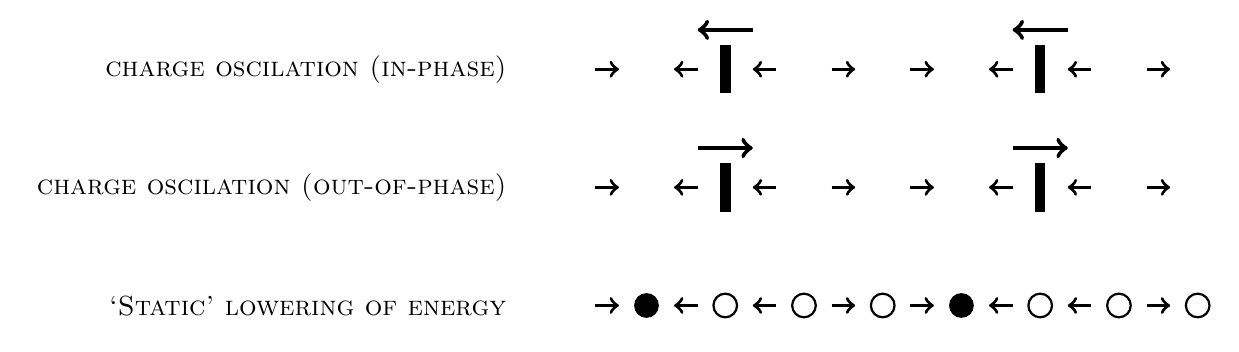
\begin{tikzpicture}
    % domain wall movement
    \foreach \y in {1.5,3} {
        \foreach \x in {0,4} {
            \draw [->, very thick] (\x,\y) -- (\x+0.3,\y);
            \draw [<-, very thick] (\x+1,\y) -- (\x+1.3,\y);
            \draw [<-, very thick] (\x+2,\y) -- (\x+2.3,\y);
            \draw [->, very thick] (\x+3,\y) -- (\x+3.3,\y);
        }
    }
    % domain walls
    \filldraw (1.59, 1.2) rectangle (1.71, 1.8);
    \draw [->, ultra thick] (1.3,2.0) -- (2.0,2.0);
    \filldraw (1.59+4, 1.2) rectangle (1.71+4, 1.8);
    \draw [->, ultra thick] (1.3+4,2.0) -- (2.0+4,2.0);
    \filldraw (1.59+4, 1.2+1.5) rectangle (1.71+4, 1.8+1.5);
    \draw [<-, ultra thick] (1.3,2.0+1.5) -- (2.0,2.0+1.5);
    \filldraw (1.59, 1.2+1.5) rectangle (1.71, 1.8+1.5);
    \draw [<-, ultra thick] (1.3+4,2.0+1.5) -- (2.0+4,2.0+1.5);
    
    % charge stripe
    \foreach \x in {0,4} {
        \draw [->, very thick] (\x,0) -- (\x+0.3,0);
        \draw [<-, very thick] (\x+1,0) -- (\x+1.3,0);
        \draw [<-, very thick] (\x+2,0) -- (\x+2.3,0);
        \draw [->, very thick] (\x+3,0) -- (\x+3.3,0);
        % charge
        \filldraw (\x+0.65,0) circle [radius=0.15];
        % afm
        \draw [thick] (\x+1.65,0) circle [radius=0.15];
        \draw [thick] (\x+2.65,0) circle [radius=0.15];
        \draw [thick] (\x+3.65,0) circle [radius=0.15];
    }
    
    \node [left] at (-1,0) {\textsc{`Static' lowering of energy}};
    \node [left] at (-1,1.5) {\textsc{charge oscilation (out-of-phase)}};
    \node [left] at (-1,3.0) {\textsc{charge oscilation (in-phase)}};
\end{tikzpicture}